\chapter{The evolution of the binary population}


In this chapter, the fragmented HL models with a completed binary population from the previous chapter are left to evolve. The binary population is monitored to evaluate the influences of membership and density on the processing of binaries in a substructured configuration. In the end of the simulation, we detect very short and very wide binaries; we detail their dynamical origins and the possible implications for binary formation.

\minitoc


\paragraph*{}

A system bound gravitationally will resist external tidal forces if it sits within its Roche radius (\citealt{BT}, \S8; \citealt{Renaud2011}). For binary stars, the condition for boundedness is given by Eq.~(\ref{Eq:density_ratio})  with $D = 3$ and setting the mean density $\rho_{bin}$ over the full Jacobi volume. Thus the question of how much the mean background density rises and  compares to the mean density of the binary has important consequences for the further evolution of the binary. The situation is made more complicated if the host's potential changes rapidly, on the  dynamical time-scale $t_{cr}$ of Eq.~(\ref{Eq:0_tcr}). 

Let us first recall the results of the collapse of an homogeneous sphere of $N$ identical stars. For this case the sphere collapses by a factor $C$ before it rebounds and evolves towards equilibrium \citep{Aarseth1988,Boily2002}. The ratio of minimum radius achieved during collapse, to the initial system radius, is a 1/3 power-law of $N$, so $ C \propto N^{-1/3}$. 
% so that rich systems become systematically denser before the growth of dynamical fragments stop the collapse.
If the total mass is conserved during the collapse, the mean background density scales as $\rho \propto C^{-3}$ and so reaches a peak value $\max(\rho) \propto N$. Based on this analysis, one would expect a strong relation between the system {\it total} mass $M = N \overline{m}$ and the rate of destruction of binary stars, especially those of large semi-major axis $a$, if and when a cluster undergoes a phase of collapse.

To investigate this effect of membership on the destruction rate, various simulations were performed: their parameters are summarized in Table~\ref{Tab:6_models}. Runs with $N$ ranging from 1500 to 80000 were sampled in such a way that ensemble-averaging  gave roughly the same Poissonian standard deviations in each case. All models underwent the binary population completion procedure described in the previous chapter, with the two reference densities 6 pc$^{-3}$ and 400 pc$^{-3}$.

The aspect of a 20k star models with high density, R20h in Tab~\ref{Tab:6_models}, is shown on the left panel of Fig.~\ref{Fig:6_Rhm}, while the evolution of its half-mass radius over time is shown on the right panel. Four epochs of interest are shown as red dots: $t_0$, the initial conditions; $t_1$, end of collapse and before the bounce; $t_2$, just after the bounce; $t_3$ 30 H.u, the system reached quasi-equilibrium. These will be reference epochs throughout this chapter.


\begin{figure}
\begin{center}
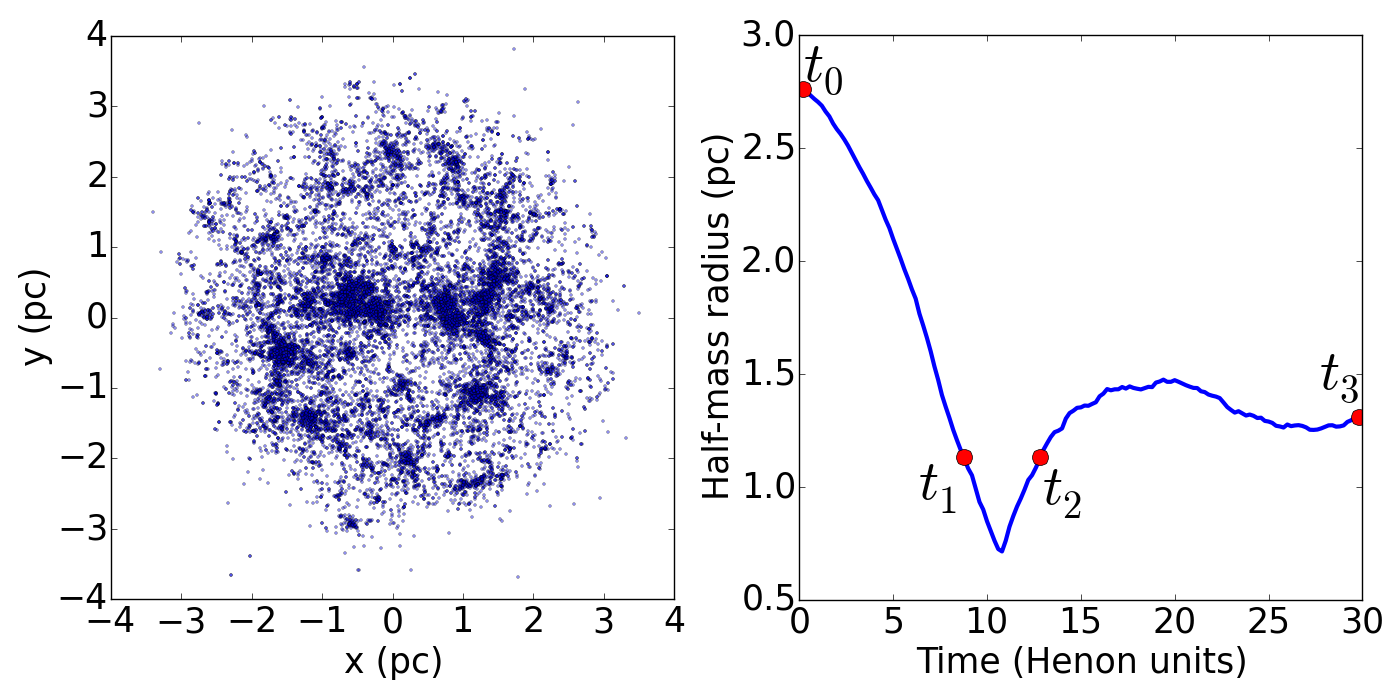
\includegraphics[width=0.9\textwidth]{Figures/6_Rhm}
\caption{Left panel: spatial distribution of a Hubble-Lema\^itre fragmented model. Right panel: evolution of the half-mass radius over time. The times labelled as $t_0$ to $t_3$ are the system configurations used in \S4 for analysis. }
\label{Fig:6_Rhm}
\end{center}
\end{figure}


% sampling of models was designed to compensate the dispersion found in low-N models and reduce the Poisson noise
%The range of $N$ covered in our study, from $\simeq 10^3$ to $10^5$,  should help quantify that relation and also
% allow to extrapolate with more confidence in the range of $N \sim 10^6$ member stars appropriate for globular clusters. 
% The tidal field of self-gravitating systems can be shown to scale with density \citep{DM91,renaud2011}.
% Therefore, one can expect the membership of a collapsing system to impact its density and tidal fields.
%
%Most previous simulations on the evolution of binary populations in star clusters considered a relatively small number of stars of the order of a thousand [ ref, parker, etc]. Going from 1500 to 80000 in our simulations allows to explore the previously uncharted territory for nbody binary evolution of young globular clusters. 

\begin{table}
\begin{center}
\caption{Summary of simulations. Starting from an HL fragmented configuration, a binary population was injected to complete the spontaneous binaries, reaching an overall binary fraction of 0.42. Densities withing half-mass radius are shown at t=0 and time of deepest collapse.}
\label{Tab:6_models}
\begin{tabularx}{0.6\textwidth}{XXlXXX}
\hline
Name & N & Sampling & $\rho_{h,0}$ (pc$^{-3}$) & $\rho_{h,max}$ (pc$^{-3}$)  \\
\hline
R1.5h & 1500 & 40 & 400 & 1.7$\cdot10^3$\\
R5h  &  5000 & 10 & 400 & 4.0$\cdot10^3$\\
R20h &  20000 & 10 & 400 & 1.4$\cdot10^4$\\
R80h &  80000 & 1 & 400 & 7.1$\cdot10^4$\\
R1.5l &  1500 & 40 & 6 & 13\\
R5l &  5000 & 10 & 6 & 79 \\
R20l &  20000 & 10 & 6 & 192 \\
R80l &  80000 & 1 & 6  & $10^3$\\
%R1.5ul & Uniform & 1500 & 40 & 6 & 2.9 $10^3$\\
%R20ul & Uniform & 20000 & 40 & 6 & 1.4 $10^4$\\
%R1.5uh & Uniform & 1500 & 40 & 400 & 3.7 $10^5$\\
%R20uh & Uniform & 20000 & 40 & 400 & 7.6 $10^5$\\
%R1.5uh & Uniform & 1500 & 40 & 400 \\
%R1.5ul & Uniform & 1500 & 40 & 6 \\
%R5uh  & Uniform & 5000 & 10 & 400 \\
%R5ul & Uniform & 5000 & 10 & 6 \\
%R20uh & Uniform & 20000 & 10 & 400 \\
%R20ul & Uniform & 20000 & 10 & 6 \\
\hline
\end{tabularx}
\end{center}
\end{table}


\section{Results}


\subsection{Total binary fraction}



\begin{figure}
\begin{center}
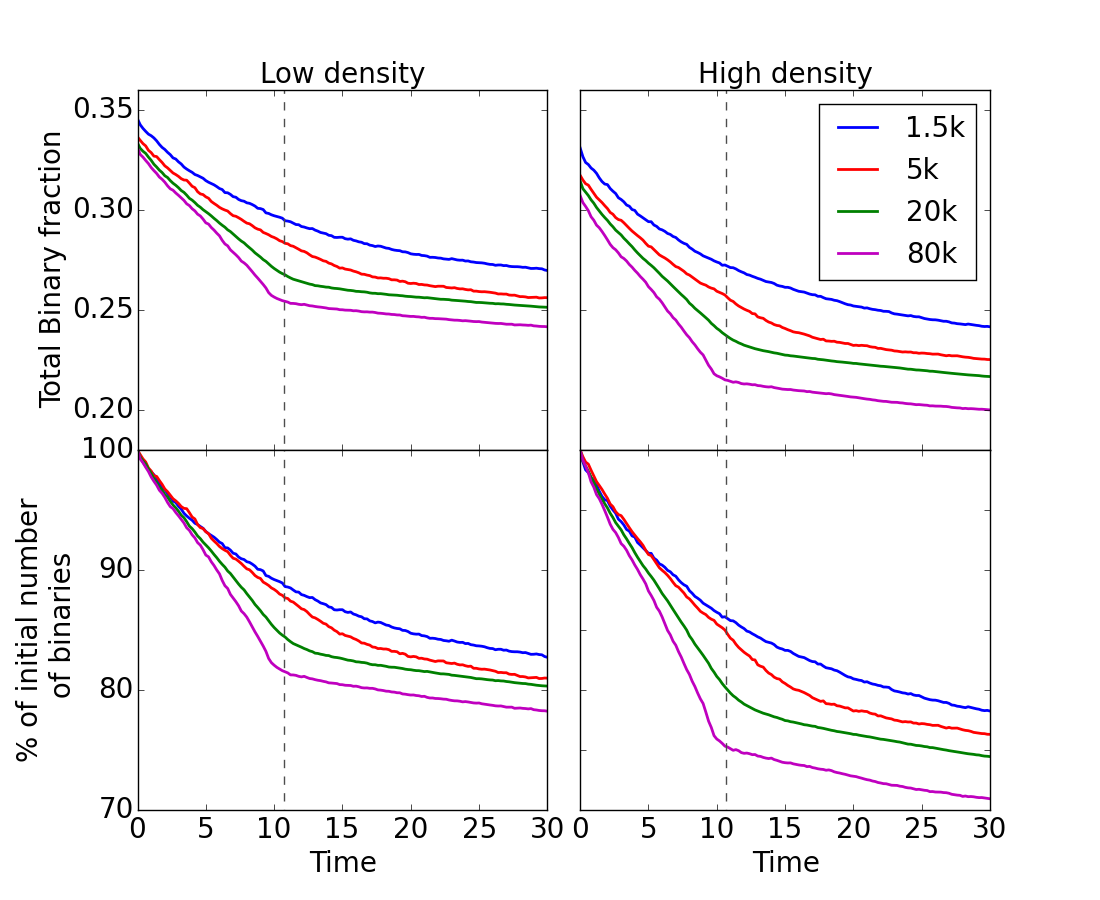
\includegraphics[width=0.8\textwidth]{Figures/6_TotBinFrac_vs_time}
\caption{ Top panels: total binary fraction over time for different cluster memberships. Lower panels: total number of binary over time compared to initial number in each system, in percentage. The vertical dashed line indicates the time of deepest collapse.  }
\label{Fig:6_TotBinFrac}
\end{center}
\end{figure}

We show on Fig.~\ref{Fig:6_TotBinFrac} the evolution of the binary fraction in HL fragmented systems as a function of time. The time when the systems rebounds from the global in-fall, $t \approx 10$ units, is marked with a vertical dotted line on each frame. The binary fraction decays in each case during the course of evolution, regardless of their membership $N$ or initial density. 
% during their collapse for several cluster memberships.
All systems display two different regimes of binary destruction, before and after the bounce from global collapse. Before the bounce, binaries are destroyed at a higher average rate, the more so for the more massive systems (large $N$). 
% before the collapse. These two regimes are more pronounced with a large number of stars in the system.
After the bounce ($t > 10$) the slopes all flatten out and binaries are continuously destroyed but at a lower rate. For example, the R80h simulation removes 2.5\% of its binaries per time unit before the collapse; this rate goes down to 0.25\% afterwards. Similarly, the low-density $N = 80$k run has  1.7\% before the collapse and 0.16 \% thereafter.


We interpret these findings as follows. In the first stages of evolution, the rate of binary destruction is driven by the two-body relaxation in the small clumps of the HL configuration. To see this, Fig.~\ref{Fig:6_TotBinFrac}, bottom row, graphs the {\it relative} fraction of surviving binaries for each model. The linear slope is virtually identical up to $t \approx 5$ units. The internal dynamics of clumps is independent of the larger system in which they are embedded.
As collapse proceeds, larger $N$ systems develop a deeper global potential well: this is easier to see for  $t \rightarrow 10$ as the curves fan out. The range, of about $10\%$,  accrued at $t = 10$  between runs of different $N$, is almost unchanged at the end of the simulations, at $t = 30$ units. 
% clumps are $\sim 10$  times more efficient at destroying binaires than a virialized spherical system. While the transition between the regimes gets blurrier and the pre-collapse regime softer with decreasing membership,
The rate of binary destruction post-bounce is practically the same for all $N$, though note that it remains higher for the high-density calculations (the final count of binaries drops from $\simeq 80\%$ at low density, to $\simeq 70\%$ at high density).

There is a clear tendency for the pre- and post-collapse transition to be sharper as $N$ increases. We interpret this in the light of Eqs. (\ref{Eq:0_tcr}) and (\ref{Eq:0_trel}).  
%  Going back to the relaxation time extimations in section \ref{Sec:Simulations},
We note that the $N = 1.5$k models are dominated by two-body interactions, the mass-segregation time-scale drops to $\sim 1$ time units, and not by the overall collapse motion that drives density upwards, destroying binaries.
  At the other end of the spectrum, the $N = 80$k  models have a global mass-segregation time-scale $>~30$ time units.  These models, like all the others,  are initially dominated by two-body interactions in  their clumpy substructures. However the later evolution sees the overall collapse motion take over.
  It is the imprint of that global in-fall which allows the density to peak at higher values (cf. Table \ref{Tab:6_models}) and laminate binaries more   efficiently around that time. Since the re-bound is of short duration, the strong tidal field drops quickly as we shift in the post-bounce phase.



\subsection{Binary fraction vs primary mass}



\begin{figure}
\begin{center}
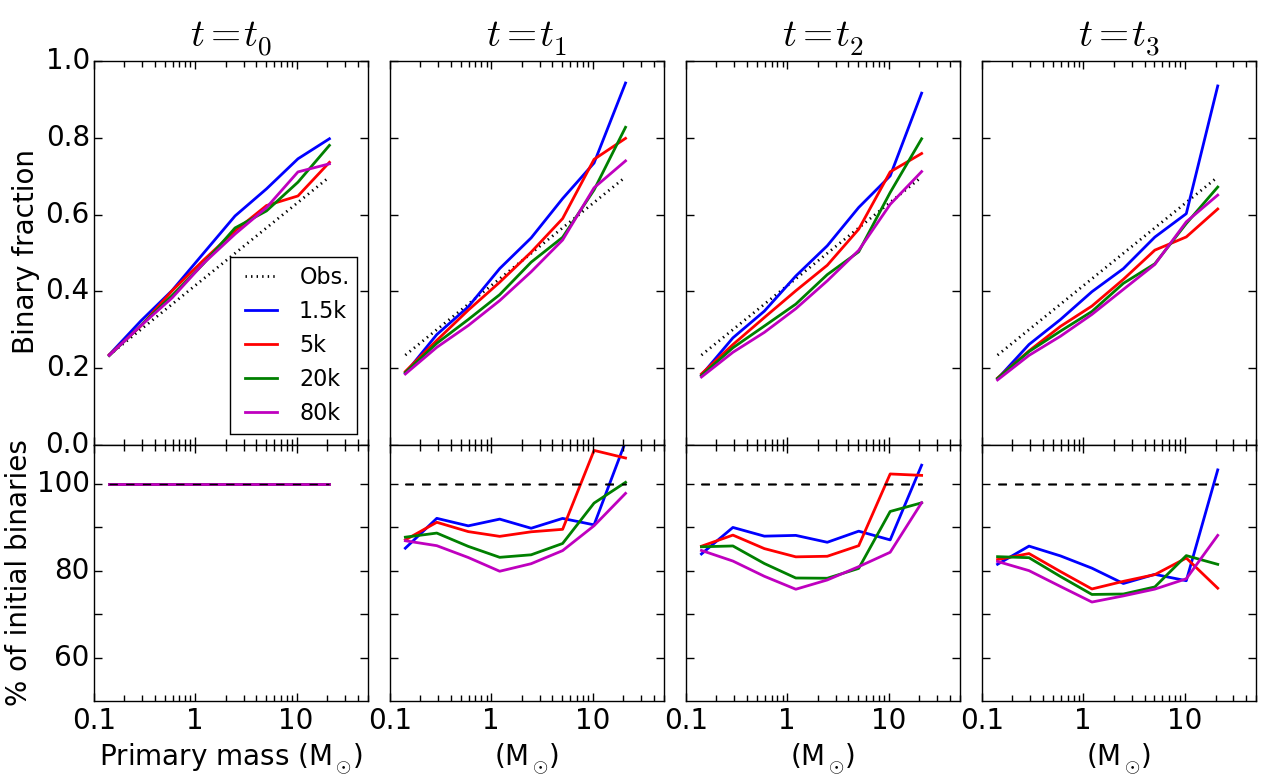
\includegraphics[width=\textwidth]{Figures/6_BinFrac_vs_mass_LD}
\caption{ The data is from low density models. Top panels show the binary fraction in logarithmic bins for the primary masses. Dotted line show the linear fit to observations shown in Fig.~\protect\ref{Fig:5_spontaneous_primarymass}. In bottom panels, the number of binaries in each primary mass bin is shown as a percentage of the initial number (t=0). The 100\% value is shown as a horizontal dashed line.}
\label{Fig:6_BinFracVsMass_LD}
\end{center}
\end{figure}


\begin{figure*}
\begin{center}
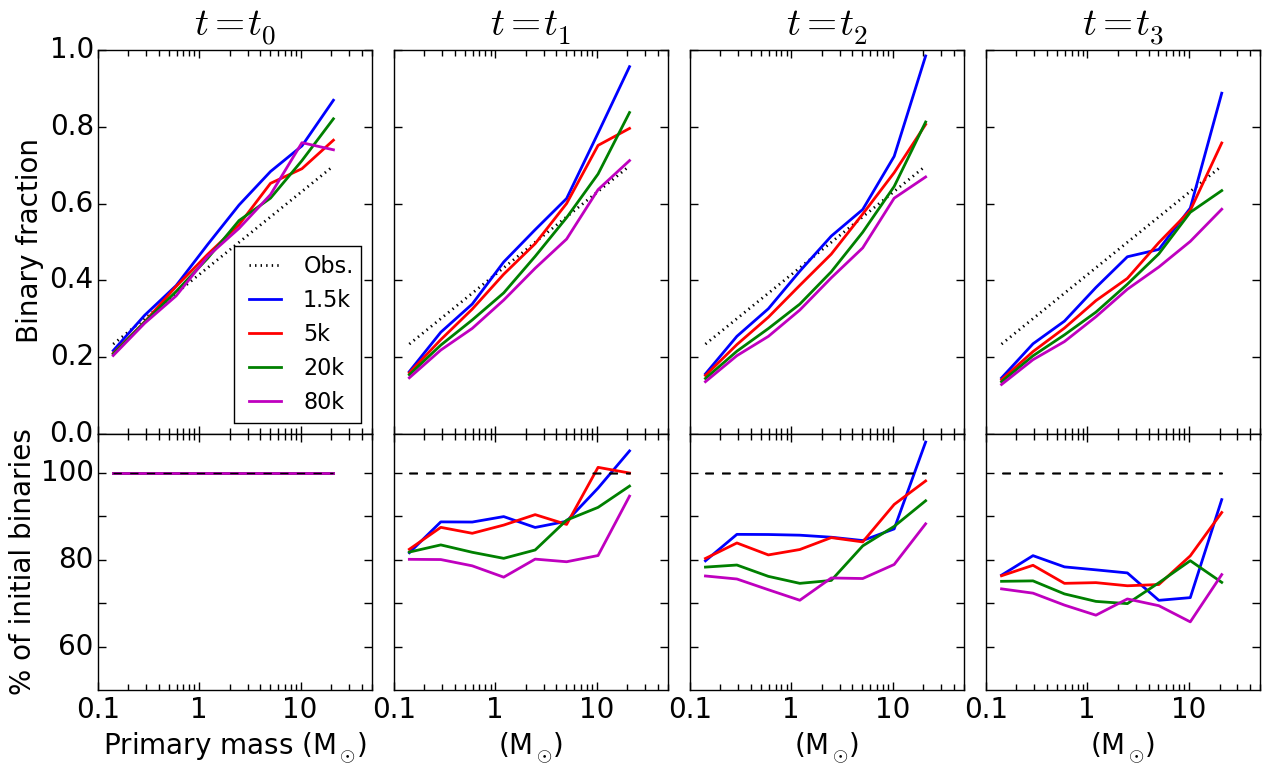
\includegraphics[width=\textwidth]{Figures/6_BinFrac_vs_mass_HD}
\caption{ The data from high density models. Same key as Fig.~\protect\ref{Fig:6_BinFracVsMass_LD}.}
\label{Fig:6_BinFracVsMass_HD}
\end{center}
\end{figure*}


% This destruction is most efficient towards low-mass primary binaries, as seen on
To determine whether the evolution affects binaries differently according to their mass, we show on Figs.~\ref{Fig:6_BinFracVsMass_LD} and \ref{Fig:6_BinFracVsMass_HD} the binary fraction in relation to the primary mass. Results are shown at four different times, and for all runs of $N$. The top row of each figure is the binary fraction $f_m$ and the bottom row the percentage of binaries with respect to the initial distribution. 
 %
%The binary fractions per primary mass bins over time and for N=1.5k,5k,20k,80k are shown, as well as the percentage of remaining binaries in each mass bins compared to t=0.
This representation highlights which binaries are the most processed in the system. The panels for $t = t_1$ and $t_2$ are for times immediately before and after the bounce (cf. Fig.~\ref{Fig:6_Rhm}). The dynamical evolution within the clumps and during the collapse impacts preferentially light-primary binaries; binaries with a more massive primary (say, $> 5 \Mo$) survive better. We stress that the trends are indicative and at the $\sim 20\% $ level in all cases. Bearing this caveat in mind, inspection of the different cases does suggest that the results for low-N runs are more the result of the internal dynamics of clumps, where star-star interactions would favour the ejection/destruction of low-mass binaries. Note how the low-N models in fact form {\it additional} high-mass binaries during in-fall, since the binary fraction exceeds 100\% at $t = t_1 $ and $t_2$. This is not so for the $N = 20$k and $80$k models, which we interpret as due to the stronger tidal fields in these models which stops new binaries from forming. It is interesting that despite the deeper infall achieved by  these large-N models, the trend of increased survival with primary mass is not eradicated: this would have been the case had the external (global) tidal field clearly dominated the binary destruction. Instead, we find that the strong fields do not erase memory of the early evolution phase of the clumpy distribution. 

% This is especially true for low-membership clusters, in which additional high-mass prim. binaries are formed, increasing the binary fraction in the last bin. In a small cluster, the stochastic star-star interactions dominates over the large-scale motion of collapse, which favors the formation of binaries, especially for massive stars which act as a potential well in the heart of clumps. 

The results for the later time $t = t_3$ displayed coincides with the end-time of the simulations. At that point all models have reached equilibrium and the binaries have been processed dynamically in such a way that the binary fraction decreased monotonically for all primary masses. It is worth noting that the low-density models (Fig.~\ref{Fig:6_BinFracVsMass_LD}) have evolved for a physical time $t \approx 18$ Myr, while the high density ones  (Fig.~\ref{Fig:6_BinFracVsMass_HD}) up to $t \approx 3$ Myr only. This may explain the greater scatter among the different runs for these models (they have more intense tidal fields but have less time to act on the binaries). We also note that the peak at high primary mass, clearly visible at $t = t_2$, is still apparent at $t = t_3$, except for the case $N = 80$k., which is the model with the highest density and the strongest tidal field. We interpret this as indicating that the wide binaries have had time to be split, while this process is yet incomplete in the other models. This view is backed up from inspection of the low-density runs at $t= t_3$ on Fig.~\ref{Fig:6_BinFracVsMass_LD}, where all the peaks seen at $t = t_2$ have been flattened save the runs with $N = 1.5$k. We believe that the more stochastic low-N runs may have produced more wide-binary escapers due to their shallower potential well. These would therefore not be processed collisionally in the final cluster and survive in isolation. 

% The influence of density appears to be limited to the extent of processing, it is not affecting its nature. The same trends are visible, only more pronounced for high density simulations. Overall, an increasing membership tends to slightly enhance binary processing, while limiting stochastic high-mass primary binary formation.


\subsection{Semi-major axis distributions}

\begin{figure}
\begin{center}
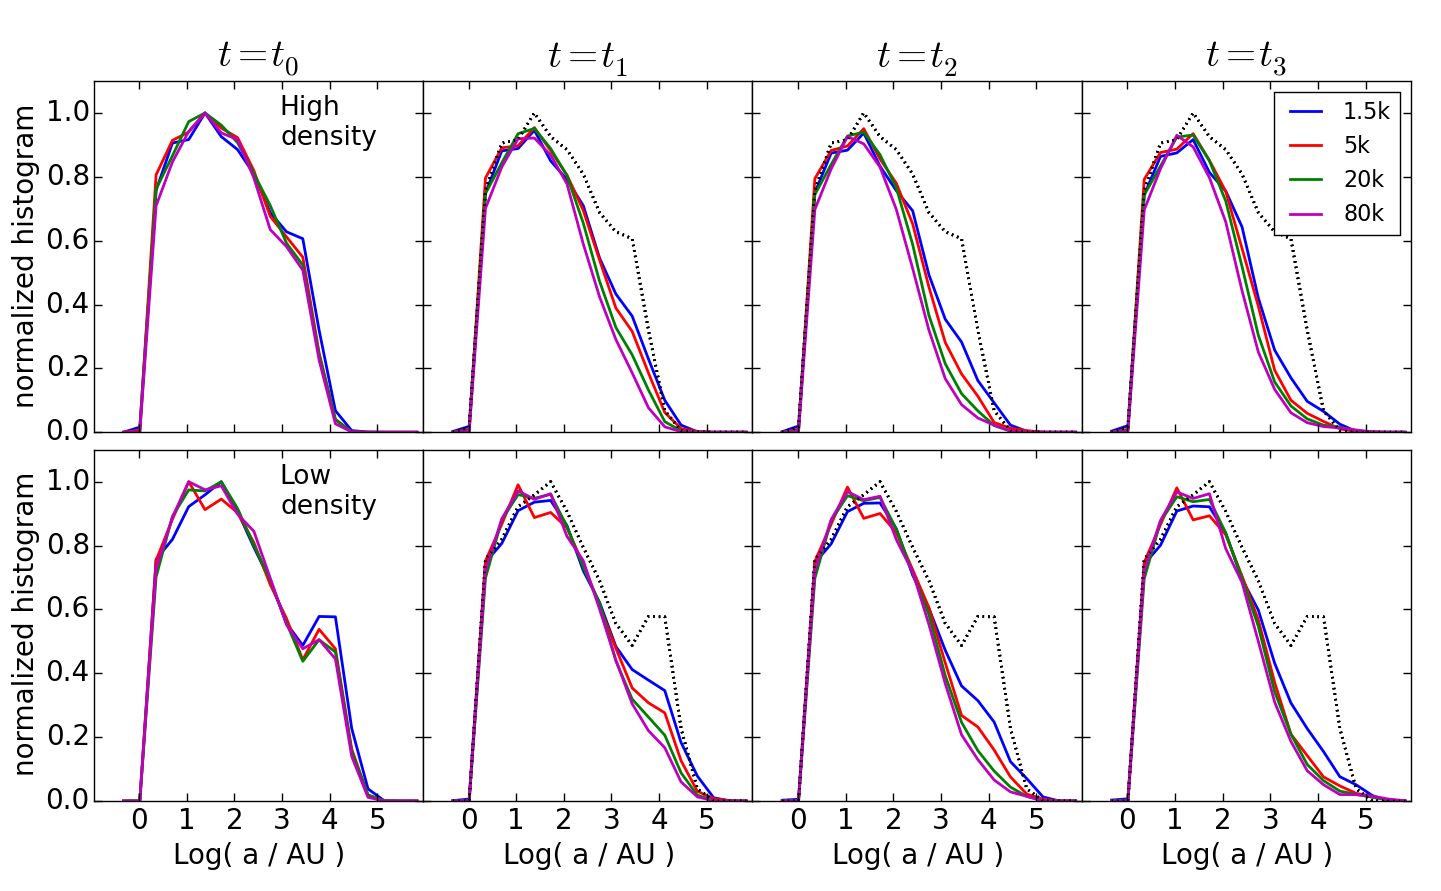
\includegraphics[width=\textwidth]{Figures/6_SMAxis_histogram}
\caption{Histograms of semi-major axes for the binary population at four different times and for four different cluster membership. The dotted black line shows the distribution of $N = 1.5$k models at $t=0$ as a reference for the initial distributions. High density models are in the top row, while low density models are in the bottom row. The reference times are taken from Fig.~\ref{Fig:6_Rhm}.}
\label{Fig:6_SMAxis_histogram}
\end{center}
\end{figure}

The evolution of the distribution of semi-major axes $a $ % (or period, separation, both directly related to semi-major axis)
in a binary population hinges on its dynamical environment. Several analytical and numerical studies
\citep{Heggie1975,Kroupa1995,Kroupa1995a,Heggie2006,Parker2009,Parker2011} have shown that wide, weakly bound binaries are preferentially disrupted, so sculpting the distribution towards tighter, more bound binaries. 
This evolution is shown on Fig.~\ref{Fig:6_SMAxis_histogram} which graphs the distribution histograms as a function of semi-major axis $a$. The distributions are plotted for four various times, membership $N$ and both the values of initial density. The averaged distribution computed from the models with $N = 1.5$k is shown as a dotted line and serves as reference. To ease the comparison between models with different $N$, all histograms were normalized to the reference initial profile at $t=0$ (e.g., the area under the curve is the same for all the models).


We first distinguish between high- and low-density models. The overall behaviour of the models is the same, with a rapid dissolution of large semi-major axis binaries,
$a~\sim~10^3$~AU or more. This takes place prior to the bounce, when $t < t_1$ but is a continued trend from the start of the computations to the end.
As anticipated, high density models (top row on Fig.~\ref{Fig:6_SMAxis_histogram}) process the binary population more efficiently, reaching deeper in the short-axis
range, down to  $a \sim$ 20 AU, compared to $a \sim$ 100 AU for the low density models.
This can be gauged qualitatively by the gap that opens up between the dotted line and the histograms.

The system mass (or membership $N$) has little influence on the evolution of the histograms, however, as the collapse factor $C$ increases with $N$, the larger $N$ models process significantly wider $a \sim 10^3$ AU binaries ; this is true regardless of the initial density (high or low). Note that, here too, the $N = 1.5$k models stand out, in the sense that their wide binary population is less efficiently processed.
%
%As is seen in the other figures, the membership does not have a strong influence, but a small trend can be seen: large clusters, though with similar density, tend to process more large and intermediate binaries than small ones during the collapse of the fragmented system. After the collapse, the trend tends to diminish, though 1.5k distributions remain slightly less processed in the large separation range.

\begin{figure}
\begin{center}
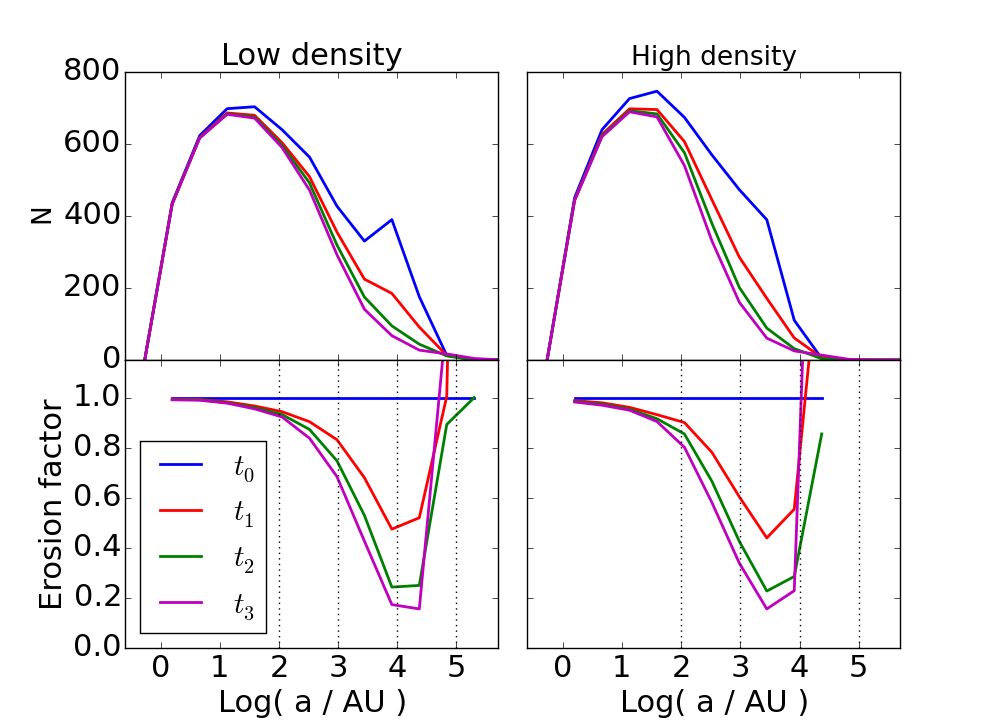
\includegraphics[width=0.75\textwidth]{Figures/6_S_shape}
\caption{Top panels: histogram of semi-major axis at four different times for the $N = 20$k  models. 
Bottom panels shows the erosion factor, the ratio between the sizes of the initial binary population and the one at a given time, in each primary mass bin. }
\label{Fig:6_S_shape}
\end{center}
\end{figure}

Having identified the mean initial density as the main driver for binary population evolution, we wish to compare the rate of survival of binaries with the analytical approach by  \cite{Marks2011}. These authors  introduced an analytic operator acting on a binary population to mimick its evolution in  a host star cluster,  dispensing with N-body simulations.  \cite{Marks2012} used this framework to reproduce the destruction of wide binaries, using the operator as an "erosion  factor" applied to a birth semi-major axis distribution, selectively reducing the number of binaries in each semi-major axis bin (see their Fig.~1 for an illustration of their approach). The erosion factor is bound to the interval $[0, +1]$, and equals one when all binaries of a given semi-major axis $a$ are retained (zero when they are all destroyed). 


 The erosion factors arising from $N = 20$k simulations for the four reference times are displayed on  Fig.~\ref{Fig:6_S_shape} (bottom panels). 
%
% Dotted lines highlight the
% $10^2, 10^3, 10^4, 10^5$ AU positions to ease the comparison between low and high density. 
The model with initially high density heats up and splits binaries of  (relatively) shorter semi-major axis  during the collapse, and beyond: the most dramatic phase of evolution between times  $t_0$ and $t_2$. During that interval,  nearly 80\% of  binaries with $a > 100 $ AU are split. There is comparatively little evolution from $t_2$ to $t_3$,  which covers the remaining {\it half} of the run time.  
The run of the erosion factor with $a$  and its time-evolution are very similar  when comparing the runs of models with  high- and low initial  density. The most striking difference is the shift of the minimum value of the erosion factor, from a semi-major axis $a \approx 3 000$ AU, to larger axes $a \approx 10 000$ AU  in the case of low density models .  The extent of the shift, a factor of $~4$, is consistent with the scaling of the mean separations between stars $ l \propto \rho^{-1/3}$; we compute for high and low density systems 
\begin{equation}
\frac{l_{low}}{l_{high}} = \left(  \frac{\rho_{high}}{\rho_{low}}\right)^{1/3} = \sqrt[3]{\frac{400}{6}} \simeq 4 .
\end{equation}

This fact alone implies that the evolution of fragmented mass profiles through a relaxation phase is driven mostly by stellar encounters. The same conclusion applies for the evolution of the  fractal models of \cite{Parker2011}. 
%  in fractal clusters undergoing cool collapse.
% cmb : shift to discussion section 
% A substructured system processes its binary population, reducing the number of binaries over time, as shown by 
The late stages of cluster formation, post-bounce and nearly in virial equilibrium, compare well with the 
analytical operator  of \cite{Marks2012}. One significant difference that this approach does not factor in is the formation of wide binaries in the post-bounce phase. The operator may still adequately compute  the evolution of a binary population in a system in global  equilibrium. Nevertheless, expanding low-density volumes and other phenomena related to the virialisation phase appear to be outside the scope of a cluster-wide binary-processing analytical  operator. 
% Apart from the uptick at large separation, the shape of the erosion factor we find is similar to the analytic operator from % \cite{marks2012}, the processing in the relaxed system appears similar. 

% \subsection{Comparison with uniform mass profiles}
\subsection{Tidal shocks} 

%\begin{figure}
%%\begin{center}
%\includegraphics[width=\columnwidth]{../Figures/SMAxis_UnifHub}
%\caption{ Comparison of the semi-major axis distribution of HL models (in blue) and Uniform spheres (in red) just before the deepest collapse ($t = t_1$, dashed lines) and just after ($t = t_2$, solid lines). }
%\label{Fig:UnifHub}
%%\end{center}
%\end{figure}

We noted how larger-N simulations tend to iron out a larger fraction of binaries (see Fig.~\ref{Fig:6_SMAxis_histogram}). 
The weak trend with increasing $N$ implies that both star-star interactions (including multiple stars) and global tidal forces both boost the heating up and unbinding of  binaries.  The shift seen on Fig.~\ref{Fig:6_BinFracVsMass_HD} is small but systematic: from 15\% for $N = 1.5$k, to 25\% for $N = 80$k of all binary stars are destroyed at the bounce ($t \approx 10 $ units).  To get a better appreciation for the trend (or lack thereof) with $N$, let us compute the energy transferred to a binary star by the tidal field. At the end of the collapse, the stars move on mostly radial orbits at high velocities. Since they cross a dense region in a short time, we make use of the tidal shock approximation developed by \citet[see also \citealt{Boily2004,BT}]{Spitzer1958}.

%Spitzer (1958)} see also \cite{Boily2004}, \cite[\S8]{BT}. 

%A higher N does mean a higher initial radius to preserve density, but this does not compensate the previous effect, and so a higher density at collapse is expected. 
Taking inspiration from the tidal shock suffered  by a cluster crossing the galactic disk, we can get an estimation of tidal heating on a binary crossing the dense center of the system at the time of deepest collapse. \cite{BT} define the change of specific binding  energy $\Delta E_s $ of a self-gravitating system of size $r$, mass $\mu$, crossing a spherical volume of projected surface density $\Sigma \approx r \rho$ at radial velocity $V_r$, as:

\begin{equation}
\label{Eq:6_DeltaEs}
\Delta E_s = \frac{14 \pi^2 G^2 \Sigma^2 r^2}{3 V_r^2}\, .
\end{equation}
We seek out the scaling of this relation with the number of stars $N$, keeping the system initial mean density $\rho(0)$ constant. This implies that the total mass $M \propto N$.  The expectation from the analysis of fragmentation modes is that the radius at the bounce $r = R_o / N^{1/3}$. The projected density at the bounce therefore scales as $\Sigma \approx M / \pi r^2 $. Ignoring mass loss and the energy dissipated by binary disruption, we can estimate the magnitude of the square radial velocity $V_r^2$ from the relation 
\begin{equation}
3 V_r^2 \approx \frac{2G M}{r} \propto \frac{N}{N^{-1/3} R_o}.
\end{equation}

Substituting in (\ref{Eq:6_DeltaEs}) and replacing $r$ by the semi-major axis, we find 

\begin{equation}
\Delta E_s =  \frac{14\pi G^2 ( M / \pi r^2 )^2 a^2}{ 2GM / r } \propto \frac{G M \, a^2}{r^3} \propto \frac{GM}{R_o^3} N a^2\, .
\end{equation}

The binding energy per unit mass of a binary star is $E_s = - G \mu / 2 a $. The relative energy imparted to the binary by the shock is therefore 

\begin{equation}
%\frac{\Delta E_s}{E_s} = \frac{0.65}{C^4} \cdot \frac{M}{m_{bin}} \cdot \left( \frac{a}{R_0} \right) ^3 
\frac{\Delta E_s }{E_s} \approx \frac{7\pi M}{\mu R_o^3} a^3 N    \, . 
\end{equation}

We chose to keep the initial mean system density constant, so that the ratio $ M/( \mu R_o^3)$ is independent of $N$. The final scaling reads  
  
\begin{equation}
\frac{\Delta E_s}{E_s}  \propto a^3 ~ N \, .
\end{equation}

An increase in membership $N$ implies more significant heating of the binary star. If we set $\Delta E_s/E_s = 1$, then an increase of $N \rightarrow 10 \times N$ should have the same relative effect on a binary of semi-major axis $a \rightarrow a / 10^{1/3} \approx a / 2.15$. 
By implication, the peak of the distributions seen on Fig.~\ref{Fig:6_SMAxis_histogram} should shift from 
$a \approx 40 $ AU to $ a \approx 40 / 3.76 = 10.64 $ AU, as we work up from $N = 1.5$k to $N = 80$k calculations. 
This shift is not seen on the figure. What we see, on the other hand, is that large-N systems tend to deplete more efficiently the wide binaries, so that at the same stage of evolution, the richer systems have a binary distribution that falls off more quickly at large separations. We attribute the weak dependence on $N$ to the approximation of a static background mass distribution\footnote{The original treatment by Spitzer fixed a thin (vertically mixed) disc crossed by a stellar cluster at high speed.}. In reality, the whole structure moves on the same short dynamical time-scale of Eq.~(\ref{Eq:0_tcr}) and hence the effective surface density $\Sigma$ is much reduced if the system as a whole begins to re-expand.  We suspected that the choice of fixed initial density may be the reason for the undetectable shift of the peak on Fig.~\ref{Fig:6_SMAxis_histogram}. Our choice of initial conditions imply that the system size $R_o \propto M^{1/3}$; had we chosen instead to use an empirical relation such as $R_o \propto M^{1/5}$ for stellar clusters \citep{Larsen2004}, then we would have found a scaling of $\Delta E_s /E_s \propto a^3 N^{7/5} $. The same rise in $N$ as before would have produced a shift from $\approx 40$ AU to 6.5 AU in the peak of the distribution, and this is still too large to go undetected. 

% Bit on uniform mass profiles .. 
%
%We now wish to show that the results that we have obtained for the dissolution of wide binaries is largely independant of the choice of mass profile. We do this by performing a few runs with a uniform density profile, inserting the same 
%initial binary population as in the HL models. The objective is twofold: firstly, to validate the scaling of the collapse factor with $N$ in the case of a full stellar mass spectrum with collisional effects ; and secondly, to see whether the stronger 
%tidal field of a uniform collapse may yet cause a shift in the peak of the distribution of separations, post-collapse.
% 
%
%
%We show on Fig.~\ref{Fig:UnifHub} the effect on the semi-major axis distribution for the HL configuration and the uniform configuration, both for high initial density, around the times of deepest collapse, $t = t_1 $ and $t_2$. 
%The distribution were normalized to the same initial number  of binaries (at $t=t_0$). The synchronised orbits of the 
%uniform sphere models lead to a deeper collapse and 
%The uniform collapse appears more violent, destroying shorter binaries for both 1.5k and 20k stars. However, the effect of membership appears almost negligible. One would expect a high N system to reach a higher central density at collapse, as its initial matter distribution is smoother. 
%
%
%\edit{Moreover, while the increase of central density is expected to scale with N, our uniform models do not fit this trend. % Looking at the values in \ref{Tab:models}, going from 1.5k to 20k only brings a factor $\sim 2$ in collapse density, instead of $\sim 13$. This is a consequence of the mass spectrum in our models, bringing two-body interaction during the collapse and increasing the velocity dispersion. This makes the collapse shallower and attenuate the density peak. These effects: shorter collapse duration and lower density compensate the destructive power of the high density core when crossed by a binary.}

\section{Extreme tight-  and wide binaries}

As mentioned in \S~\ref{Sub:spontaneous_separations}, \cite{Bate2012} has found several examples of binaries reducing their separation over time through stellar encounters, from $\sim 10 $ AU down to $ \lesssim 0.5 $ AU. Tighter systems were hindered by numerical resolution issues. The regularised treatment of close encounters (which allows to integrate up to machine precision) of the code NBODY6 means that the same collisional process will be at play in the calculations that we have performed. Since no binaries with semi-major axis $a$  shorter than $ 1 $ AU was inserted in the initial conditions, we focus first on the statistics of binaries that evolved to $a < 1 $ AU. In the second part of this section, we will explore the formation and the evolution of very wide ($a > 10^4$ AU) binaries, many of which end up loosely bound to the stellar cluster  as a whole.   
% We wanted to see if such behaviour was found in our systems. No binaries shorter than 1 AU was injected, we looked at 
% all binaries with separation smaller than this.

\subsection{Tight binaries}

\begin{figure}
\begin{center}
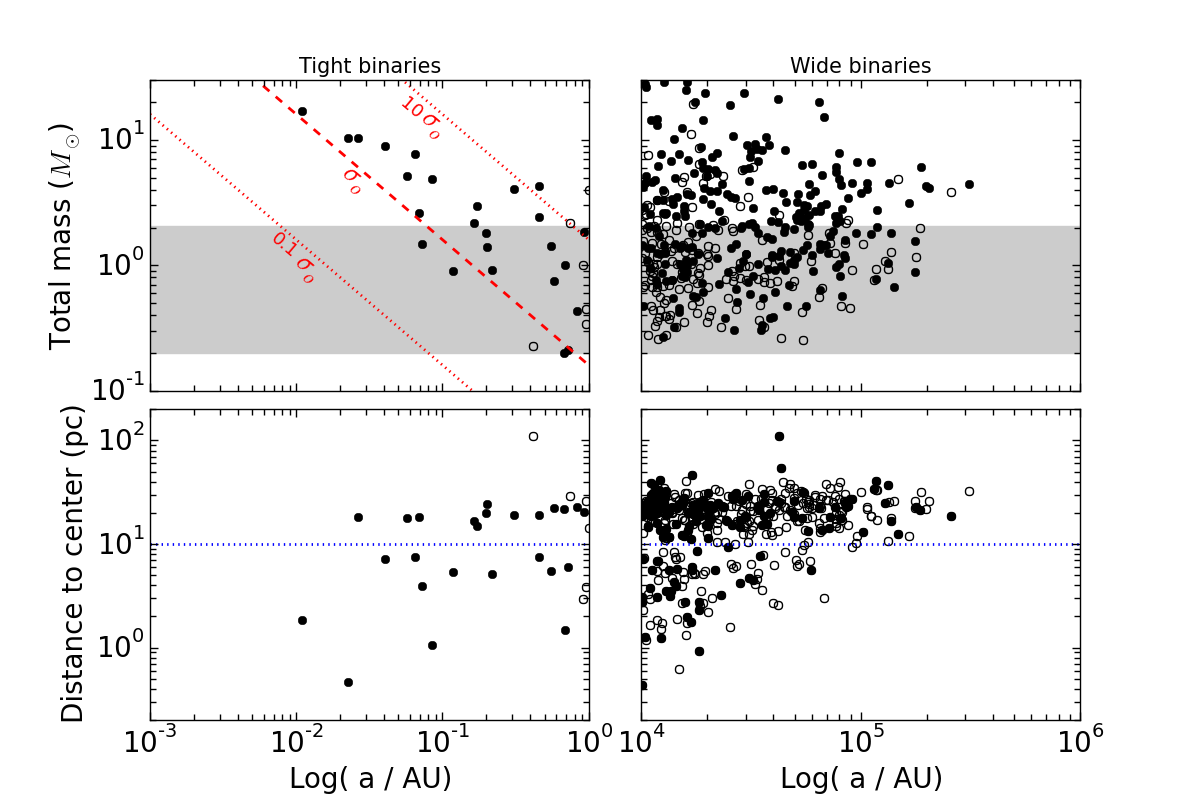
\includegraphics[width=\textwidth]{Figures/6_extreme_binaries_LD}
\caption{ Left panels: Total binary mass (top) and distance to center of the cluster (bottom) versus the semi-major axis for binaries tighter than 1AU at the end of the simulation. Right panels: same layout for binaries wider than $10^4$AU. The greyed area in the top panels shows the 90\% probability range of a binary total mass from random pairing given the present IMF. The  red dashed line in the top left panel shows the relation for  constant $v^2_\infty \sigma_{coll} \equiv \sigma_0$; it is bounded by two dotted curves that have 10$\sigma_0$ (above) and 0.1$\sigma_0$ (below). The horizontal dotted line in the bottom panel indicates the boundary between the ejecta (distance to center $>$ 10pc) and the central system. Open circles are binaries which already existed at t=0. The data is from 10 simulations of $N = 20$k stars with initial mean density of $6 /\pc^3$.}
\label{Fig:6_extreme_LD}
\end{center}
\end{figure}

Several binaries with $a < 1 $ AU were detected at the end of the low-density simulations. By comparison, almost none developed in the high-density runs. Their properties are summarised in the left panel of Fig.~\ref{Fig:6_extreme_LD}. 
The data is taken from $N = 20$k runs but similar statistics were obtained for the other setups. 
The top row shows the binary mass as a function of semi-major axis, while the  bottom row on that figure  graphs the distance of their barycentre to the center of the cluster. Open circles denote binaries that already existed at t=0, and became tighter over time, while filled circles are {\it new} binaries that formed in the course of the simulation. Inspection of these new, tight  binaries shows that {\it both} of their components were part of  binaries originally inserted in the system. Thus all new tight binaries shown on Fig.~\ref{Fig:6_extreme_LD}  are the results of strong binary-binary interactions leading to splitting or exchange. (None of the original  binaries that survived 	to the end of the simulation had  $a < 1/2 $ AU.)
	
%	 $a< 1$AU, down to $\simeq 10^{-2}$ AU, or 2 solar radius, practically a contact binary. These systems appears to 
%  follow a trend of decreasing separation for increasing total mass.
 
The statistics of these events should be compared with expectations based on estimated collision rates. 
The  time-scale for direct collisions between  particles in a self-gravitating system  depends on the degree of gravitational focusing of the colliding bodies  (\citealt[section 7.5.8, Eq. 7.195a]{BT}). This is given quantitatively by the Safronov number $\Theta = v_\star^2/4\sigma^2 = G M / (4\sigma^2 a)$, where we have replaced the surface escape velocity $v_\star$ of a single star by the 
unbinding velocity $v^2 = GM/a$ of a binary of total mass $M$ and separation $a$. To obtain an estimate of $\Theta$, 
we looked at typical clump parameters from the $N = 20$k 
R20l models: an average membership of $N_c \sim$ 50 stars and mean half-mass radius $r_{h}\sim 0.2$pc yield  
 an internal velocity dispersion (subtracting the binaries' internal motion) $\sigma \sim$ 0.5 km.s$^{-1}$.
 Setting a binary mass $ M > 2 \Mo$ and semi-major axis $ a = 1 $ AU yields $\Theta \simeq 3 700 \gg 1$. The collisional rate $\tau_{coll}^{-1}$  for binary disruption is then: 

\begin{align}
\tau_{coll}^{-1} &= 16 \sqrt{\pi} n \sigma a^2 \Theta \nonumber\\
			&= 8\times 10^{-4}~ \textrm{Myr}^{-1} \frac{n}{700 \textrm{pc}^{-3}} \frac{0.5 \textrm{km.s}^{-1}}{\sigma} \frac{a}{\textrm{AU}} \frac{M}{2 \textrm{M}_\odot}
\end{align}
with $n$ the stellar number density  $\sim$ 700 pc$^{-3}$. 
This rough estimate of the collision rate should be interpreted as a lower limit because in practice $a > 1 AU$ and many binaries have a total mass $> 2 \Mo$. We find  $\tau_{coll}^{-1} \sim 8\times 10^{-4}$ collisions per clump per Myr. Since on average $\simeq 150$ clumps formed in each R20l run, and assuming that the collision rate is 
constant throughout the 6 Myr  in-fall time, then we expect of order $O(1) $  hard  encounters  per $10^4$ stars. If most of these interactions lead to  the disruption of the binaries, some others  will result in exchange and tighter components. 

These statistics are in good agreement with % our finding of $O(20)$ events cumulated over a sample of 10 runs. 
the identification                                           % of {\it all} new tight binaries found 
in the ten $N = 20$k runs  of a total of $24$ binaries with $a < 0.6$~AU, for an average of $2.4 / 5 000  \approx 0.05 \% $ of all {\it  binary} stars  
  ($f_b \approx 1/3$ at t = 0).  The very tight binaries each have a combined mass exceeding $2 \Mo$ with a  low mass ratio $q$, ranging from 0.01 up to 0.2. It is important to mention that main sequence binary stars with a separation 
  $a \lesssim 0.02$ AU would be \textit{contact} binaries when both members are solar-type or more massive stars. 
  Clearly the evolution of such object (and in fact their formation process) calls for hydrodynamical effects that were not 
  included in our study. It is therefore remarkable that contact binaries should form strictly through gravitational scattering 
  on such short timescales. 
  

%{However, more pre-existing binaries were observed to be slightly hardened in the high density models. This latter observations can be directly explained by the higher overall density, as it increases the number of interactions, but then, why are there less new tight binaries ?}

% These objects form from binary-binary collisions. 
%\edit{A similar calculation on the core of the relaxed system yielded a similar value, however the core contains about 10\% of all stars, while 50\% of stars were initially contained in a clump, thus we expect more collisions to happen in the clumpy environment.}

 These results apply to runs with initial mean number density of $6 / \pc^3$.  The same analysis carried out for the higher 
 density models give a different outcome. 
For these models, the initial density is larger by a factor $\sim$ 60 and the velocity dispersion  by a factor $\sim$ 2, 
for all stars. From (\ref{Eq:6_CollisionalSigma}),  we find a collisional rate  $\sim$ 30 times higher than previously. 
If direct collisions were 
the main channel for the formation of tight binaries, the number of events should  increase in the same proportions.
However, inspection of the simulations yielded only 4 tight binaries, each  with a semi-major axis $a \gtrsim 0.1$ AU. 
 Thus the rate of formation of tight binaries drops to 0.4 per 5000 binaries, or 0.008\%, a six-fold decrease. 
We argue that two factors hinder the formation of these objects in high density environment. First, \cite{Geller2015} pointed out  that exchange encounters between single stars and binaries are not instantaneous (see also \citealt{Hut 1983}). 
 The process can be perturbed by other stars, so modifying the outcome of the collisions. This is also true for binary-binary collisions: casual inspection of the time series of (tight) binary stars showed that their mean separation keeps evolving 
 throughout the evolution of the model, which suggest that the binaries are part of a small-N hierarchical system. 
  It is reasonable to  expect that more hierarchical systems will develop in a higher-density environment (involving more stars) 
  and so the exchange process may never have time to take place.

Secondly, the binary exchange binary cross-section is sensitive to the impact velocity. The lack of a detailed theoretical framework on binary-binary collisions makes it difficult to pin down statistical expectations with precision. In the case of a disruptive encounter between a binary + single stars, extensive 
analytical work by \cite{Mikkola1983,Mikkola1984a,Mikkola1984b} and numerical scattering experiments (e.g., \citealt{Heggie1996,Fregeau2004})  % divided the problem into special and idealized cases (identical masses, low binding energy ratio, etc). However, 
lead to a rough estimate of the effective scattering cross section $\sigma_{bin}$ in relation to the mass and separation of identical binaries: % dependance on mass and separation can be extracted from these studies:
\begin{equation}
\sigma_{coll} \propto \frac{m_t a}{v_\infty^2}\, . 
\label{Eq:6_CollisionalSigma} 
\end{equation}

In this equation, $\sigma_{coll}$ is the effective collisional cross-section for disruption in binary-single  interactions, and $v_\infty$ is the relative velocity at infinity (prior to the collision) $\approx $ the clump velocity dispersion. Taking $ v_\infty \approx \sigma = $ constant independent of mass and binary separation, we may use (\ref{Eq:6_CollisionalSigma}) to relate binary mass $M$ to separation $a$ and  cross-section $\sigma_{coll}$. 
\cite{Hut1983,Hut1983b} gave analytical expressions for the \textit{exchange} cross sections, which scales as the above scattering cross-section at low velocities, but becomes steeper for higher velocities:

\begin{equation}
\sigma_{ex} \propto \frac{m_t a}{v_\infty^6}\, . 
\label{Eq:6_ExchangeSigma} 
\end{equation}
  
As the encounter velocity increases, it becomes harder and harder to perform a successful exchange. The two initial mean 
densities that we picked may therefore cover the transition from low- to high-velocity regimes, and reduce the number of tight binaries created to just a handful. 

Going back to Fig.~\ref{Fig:6_extreme_LD}, we plot the relation $v^2_\infty \sigma_{coll} \equiv \sigma_0$ of (\ref{Eq:6_CollisionalSigma}) as straight red lines on the top-left panel. Two dashed curves bracket a curve in full type, each with a value of  $\sigma_{coll}$ differing by a multiplicative factor of ten (increasing from the lower curve, up).  The large separations between the curves and the clustering of data points along the full curve indicate how a single value of $\sigma_0$ effectively cuts through the diagramme in two well-delimited regions.  
Thus the trend of binary mass increasing as $M \propto 1/a$ for the most tight binaries is consistent with a constant product of $\sigma_0 = v^2_\infty \sigma_{coll}$ at the time of formation. 

% A possible interpretation of this trend is that exchange binaries preserve,

%once they have formed within clumps,   
%% born hard, 
%get hardened through repeated  interactions with surrounding stars. 
%This goes on until such a time that their cross-section becomes
 %so small, that the rate of high-energy interactions drops significantly, and their 
 %hardening stalls for the reminder of the collapse. The imprint of an optimal effective 
%   cross-section would materialise itself as an inverse mass-separation correlation  on Fig.~\ref{Fig:extreme}. 
% \footnote{The evolution for a time interval $t \simeq 7 $ Myr in the smoother, post-collapse cluster mass profile does not %result in much evolution of the hard binaries, which would become once again significant on a longer, core-collapse 
% time-scale $t \sim t_r$ (cf. Eq.[\ref{Eq:tr}]). } 
 
% However, the large population of $a>1$ AU do not undergo significant hardening, the new tight binaries likely formed with their present semi-major axis. The correlation is then directly related to binary-binary exchange processes that have not been investigated in depth in the litterature for numerical reasons.
 

%\cite{ A mon avis ce n'est pas essentiel / ça été intégré ailleur dans la description de leur formation .. pour le mémoire ?? } 
%\paragraph*{Je ne sais pas trop où caser ça, peut etre plutot dans la discussion, quand on parle du fait qu'elles font partie de systemes multiples ?}  
%\paragraph*{}
%\edit{Looking in more details at the dynamical history of these 24 binaries, we can detail their formation scenarii. One is a shortened primordially existing pair, 13 formed through binary-binary collision and exchange, of which 4 happened in the clumpy configuration. The remaining 10 were the outcome of both short and long-live high order multiple systems, spawned from the splitting of binaries inside pre-existing spontaneous pairs. These systems either decay to form the short pairs, or "flicker", as the binary detection algorithm alternatively pick original parent binaries or the new short pairs, indicating chaotic evolution of small-N systems.}
%  
 
	
\begin{figure}
%\begin{center}
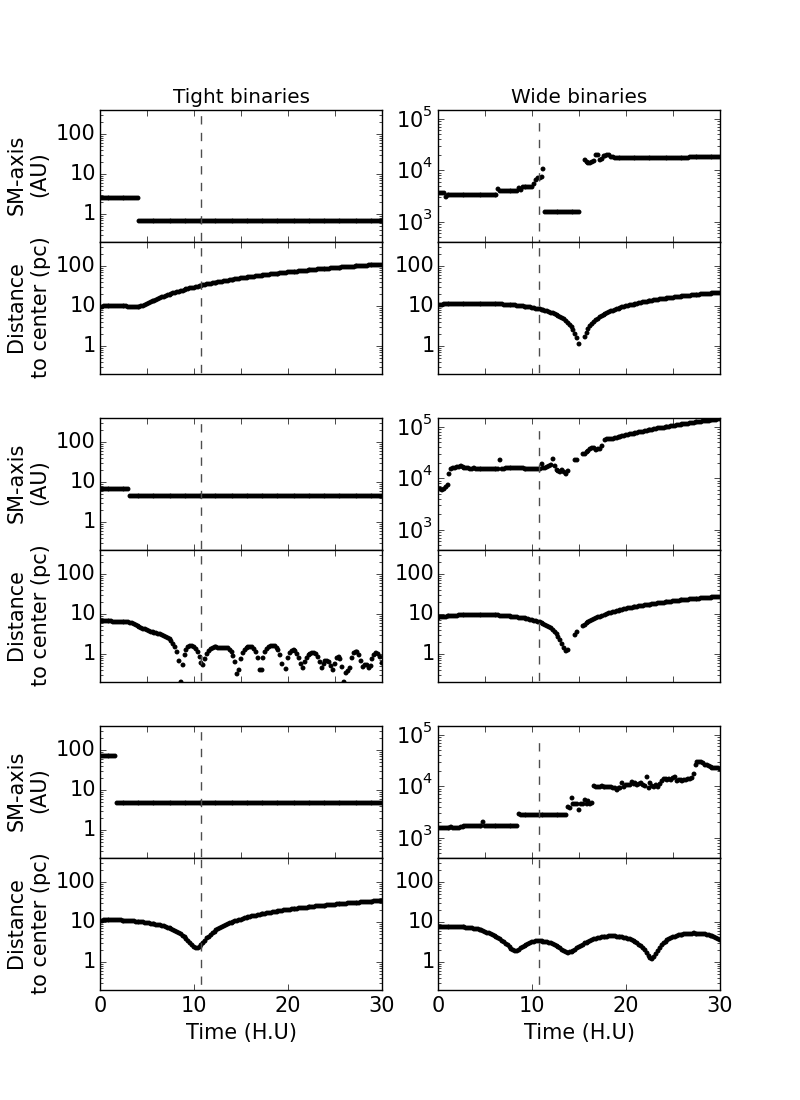
\includegraphics[width=0.6\textwidth]{Figures/6_adventures}
\caption{ Evolution of individual binaries semi-major axis and distance to center over time in the low density 20k particles models. The vertical dashed line marks the moment of deepest collapse $t \simeq (t_1 + t_2) / 2$. }
\label{Fig:6_adventures}
%\end{center}
\end{figure}


\subsection{Wide binaries}


The formation of wide `spontaneous' binaries during the HL fragmentation process leads one naturally to expect that more wide binaries will form in the post-collapse evolution of the system, when expanding streams of stars emerge from the compact bounce to form a tenuous halo. We already noted how the erosion factor on Fig.~\ref{Fig:6_S_shape} shoots up for large semi-major axes, exceeding unity at the later stages of evolution in both high- and low density calculations. This implies either that a sub-set of wide binaries got softer over time, or that new binaries of separation $> 10^4$ AU formed during the virialisation phase. If we compare the numbers for axes $a > 5.10^4 \textrm{AU} \simeq 0.25$ pc and for all ten $N = 20$k models, then there were 120 binaries more  in this range at the end of the simulations, then right after the bounce, at time $t = t_2$.  Of those 120, some forty new binaries formed in the expanding volume, while eighty are  soft binaries that became softer as a result of collisional evolution, the well-known Heggie law \citep{Heggie1975,Hills1975}. While these numbers of very wide binaries  are very low indeed, a ratio of 120 per $10 \times 20$k  stars (0.06\%), they are still significant because they would be associated with neighbouring star-forming regions, and  may yet register as correlations in phase-space coordinates. 
  

The right-hand panels of Fig.~\ref{Fig:6_extreme_LD} graph the basic properties of this sub-set of extreme wide binaries. We selected all  binaries with separations exceeding $10^4$ AU, the largest semi-major axes that were found in the initial conditions. Hence all data points shown here are the result of some evolutionary mechanism. The horizontal dotted line on Fig.~\ref{Fig:6_extreme_LD} marks a distance of $10$ pc as the separation between the central  equilibrium cluster and the volume where weakly bound ejecta orbit. Close to $\approx 60\% $ of wide binaries are escaping the main clusters or are very weakly bound to it.   Therefore most of them would be lost to the tidal field in a real cluster environment.  
 

We stress that the semi-major axis $a$ of an individual binary star is not a monotonous function of time. 
%this result is well-known for the case when a star cluster is in equlibrium, however the same rule applies to a configuration of arbitrary 
%%geometry, and independently of the evolution of the global potential.  
Fig.~\ref{Fig:6_adventures} graphs the evolution of six perturbed binaries, 3 tight and 3 wide binaries. 
Tight binaries mostly suffer strong interactions early on, before the collapse, inside a clump. This would take place  most likely at the centre of the clump, where the density is higher. What happens next is hard to predict, as the pair can then be ejected from the system by this interaction (e.g. the first binary, top panel); or  sink at the center of the cluster and remain there (second binary, middle frame); or follow the bulk of the ejecta,  falling once through the core and then leaving the system without further strong interactions  (third binary, bottom row). 
Most wide binaries experience several strong interactions. Many of these  % most feeding energy into the pairs, 
take place around the time of the collapse, as they orbit  through the dense core of the cluster. These repeated strong 
interactions will lead to heating and result in binary splitting. That is also why  
no (spontaneous) wide binary was found in  the  dense  clump cores of the initial HL configuration; instead, they form in the low-density inter-clump space. Practically all wide binaries had a first strong interaction during the densest phase of the in-fall ($t_1 < t < t_2$). 
